\section{TIG Design}
\justify{The TIG Stack is built over K8s\footnote{https://github.com/lsst-it/gi-k8s}, but for servers, a telegraf service agent needs to be setup in each one. To accomplish this, the server's configuration was performed through puppet, which is a software configuration management tool that includes its own declarative language to describe the system configuration.}
\vskip 2cm
\begin{figure}
  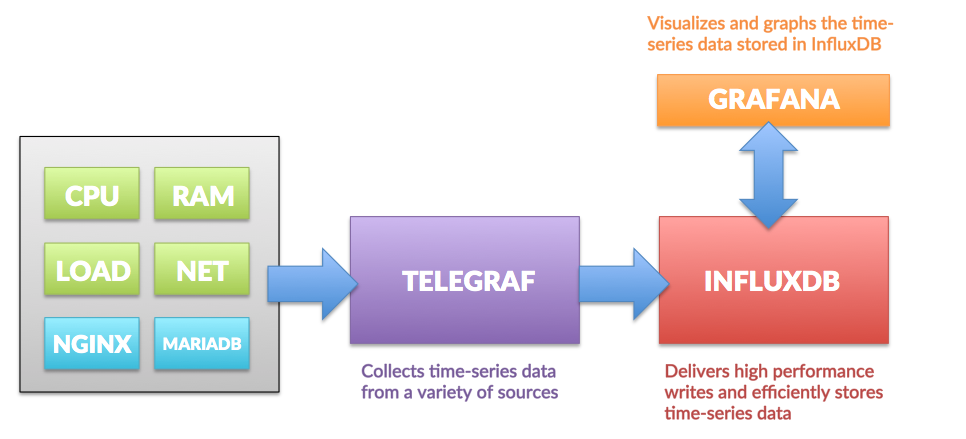
\includegraphics[width=14cm]{images/image1.png}
  \centering
  \caption{Telegraf, InfluxDB, and Grafana operational diagram}
\end{figure}
\vskip 2cm
\justify{As the diagram shows\footnote{https://www.jorgedelacruz.es/2020/11/23/en-busca-del-dashboard-perfecto-influxdb-telegraf-y-grafana-parte-i-instalando-influxdb-telegraf-y-grafana-sobre-ubuntu-20-04-lts/}, Telegraf picks up the metrics - such as CPU, RAM, Network Traffic, Load - and send them over InfluxDB. InfluxDB stores the metrics into a DB, to then be read by Grafana, which is capable of display real-time dashboards and plots.}

\newpage
\section{Telegraf Puppet's configuration}
\justify{On every server, the following puppet profile configuration is passed:}
\begin{lstlisting}
class { 'telegraf':
  hostname => $facts['networking']['fqdn'],
  outputs  => {
    'influxdb' => [{
        'urls'     => [$url],
        'database' => $database,
        'username' => $username,
        'password' => $password,
    }]
  },
  inputs   => {
    'cpu'    => [{
        'percpu'   => true,
        'totalcpu' => true,
    }],
    'mem'    => [{}],
    'io'     => [{}],
    'net'    => [{}],
    'disk'   => [{}],
    'swap'   => [{}],
    'system' => [{}],
  }
}
\end{lstlisting}
\justify{This will signal the server to install the latest telegraf package, setup the configuration file with the provided fields and ensure that the Telegraf's Service is running. All the metrics are then send to InfluxDB to be process and store.}

\newpage
\section{Telegraf over K8s}
\justify{On the other hand, network devices are not capable - at the time - of running telegraf as a service, so to be able to fetch the network device's metrics, a Telegraf intance is needed. In terms of reliability, it's better to have it over k8s than a VM. For this deployment, the following yaml charts were used:}
\begin{itemize}
  \item \textbf{ConfigMap:} Passes the content for the \textit{telegraf.conf} file to the Pod.
  \item \textbf{Deployment:} Generates a Pod with a container that runs the telegraf docker image.
  \item \textbf{Role:} A Role to run telegraf.
  \item \textbf{Service Account:} Allows the telegraf service to run under the specified service account.
  \item \textbf{Role Binding:} Links the telegraf Service Account with the Role
  \item \textbf{Service:} Creates and manage the telegraf service, as it would a Linux OS.
\end{itemize}
\section{InfluxDB over K8s}
\justify{To deploy InfluxDB service, similar kind of charts are needed, with the exception that it needs a PV to save all gathered data:}
\begin{itemize}
  \item \textbf{ConfigMap:} Passes the content for the \textit{influxdb.conf} file to the Pod.
  \item \textbf{Ingress:} Enables an entry in the Load-Balancer so that the Ingress Controller can listen incoming requests.
  \item \textbf{Job:} Even though jobs are usually to be run periodically, this one is meant to initialize the database and user.
  \item \textbf{Service:} Creates and manage the influx service, and uses the ingress to listen on ports 8086 (api calls) and 8088 (rpc).
  \item \textbf{StatefulSet:} Creates and ensures that always at least X number of replicas of the Pod are running.
  \item \textbf{Service Account:} Allows the influxdb service to run under the specified service account
\end{itemize}

\newpage
\section{Grafana over K8s}
\justify{Since Grafana is the frontend and is the one that handles users interactions, authentication needs to be managed. It also needs cluster services as well as a single-servers configurations role binging:}
\justify{
\begin{itemize}
  \item \textbf{ConfigMap:} Passes the content for the \textit{grafana.ini}and \textit{datasources.yaml} file to the Pod. Datasources file has the information from the previously deployed InfluxDB instance.
  \item \textbf{Deployment:} Generates a Pod with a container that runs the grafana docker image.
  \item \textbf{Cluster Role:} A Cluster-Wide Role to handle the grafana service.
  \item \textbf{Service Account:} Allows the grafana service to run under the specified service account.
  \item \textbf{Cluster Role Binding:} Links the Service Account with the Cluster Role.
  \item \textbf{Role:} A Role to run grafana.
  \item \textbf{Role Binding:} Links the Service Account with the Role.
  \item \textbf{Pod Security Policy:} Are fine-grained authorization for the por creation and updates.
  \item \textbf{ldap.toml:} Provides the configuration for the \textit{ldap.toml} file, that it's passed through the ConfigMap to the Pod
\end{itemize}
}
\newpage